\chapter{High-Contrast Sub-Rayleigh Imaging}
\label{sec:astrophysical_metrology_spade}
\label{ch:astrophysical_theory}

This chapter introduces the optical-imaging problem that motivates the application considered later in the thesis. Its purpose is deliberately limited: it establishes the high-contrast, sub-Rayleigh regime; explains why a conventional intensity image is statistically inefficient there; and introduces spatial-mode demultiplexing (SPADE) as the standard measurement idea. It does not yet analyse the QFI of the receiver, prescribe the estimation method developed in this thesis, or describe a particular experimental calibration.

\section{The high-contrast imaging problem}

Directly observing a faint object close to a bright one is a central problem in astronomical imaging. An exoplanet next to its host star is the motivating example, but the same statistical structure occurs for an unequal binary star or, more generally, for two incoherent point sources of very different brightness~\cite{Santamaria2024single}. Besides detection, the quantities of interest can include the angular displacement of the faint source and its brightness relative to the bright source. These are needed to localise and characterise the object.

Let $I_A$ and $I_B$ denote the detected intensities of the bright source $A$ and faint source $B$. We use
\begin{equation}
    \epsilon \coloneqq \frac{I_B}{I_A+I_B}, \qquad 0<\epsilon\ll1,
    \label{eq:intensity_ratio_epsilon}
\end{equation}
as the faint-source fraction. The more usual contrast ratio is $I_B/I_A=\epsilon/(1-\epsilon)\simeq\epsilon$ in the high-contrast limit. The separation in the telescope image plane is denoted by $\boldsymbol d=(d_x,d_y)$, with $d=\lVert\boldsymbol d\rVert$.

\todo[]{insert image of the epsilon and d in the exoplanet star binary syustem marghes job}

The difficulty has two coupled origins. First, $\epsilon$ can be extremely small: the relevant photon stream is dominated by the star. Second, the images of the two sources can overlap strongly because every finite aperture produces a diffraction-limited point-spread function (PSF). When $d$ is comparable to, or below, its width $w_0$, a faint planet does not appear as a visibly separate spot. It produces only a small deformation of the bright star's image.

\begin{figure}[htbp]
    \centering
    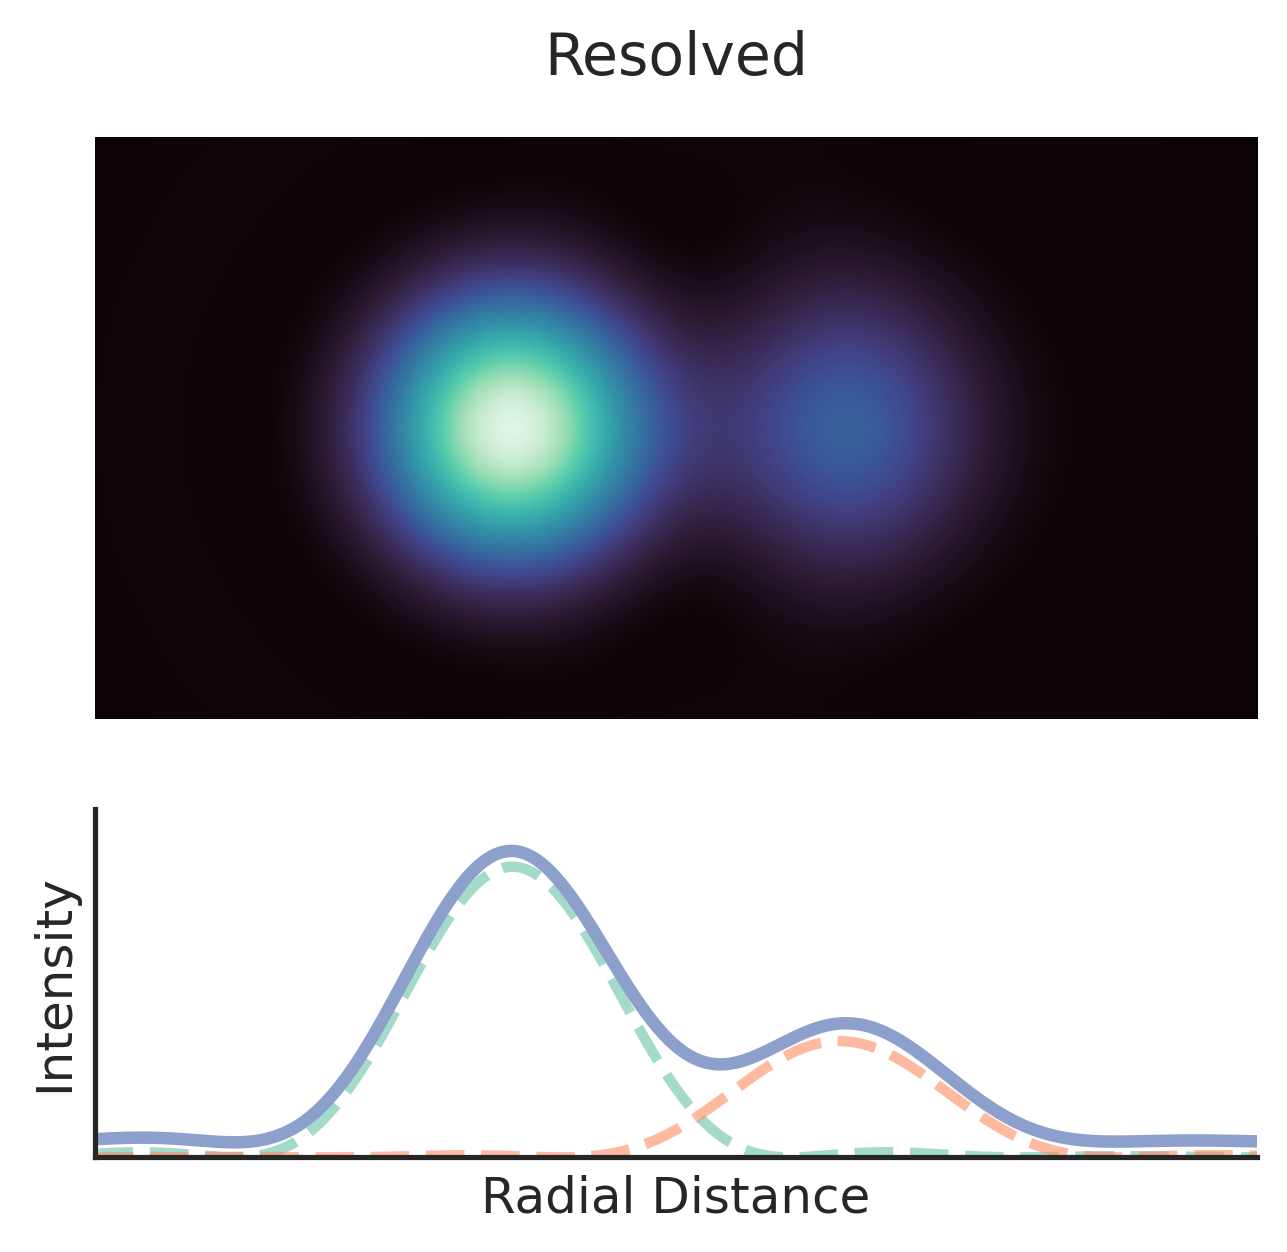
\includegraphics[width=0.48\textwidth]{figures/scripts_for_figures/rayleigh_resolved.png}\hfill
    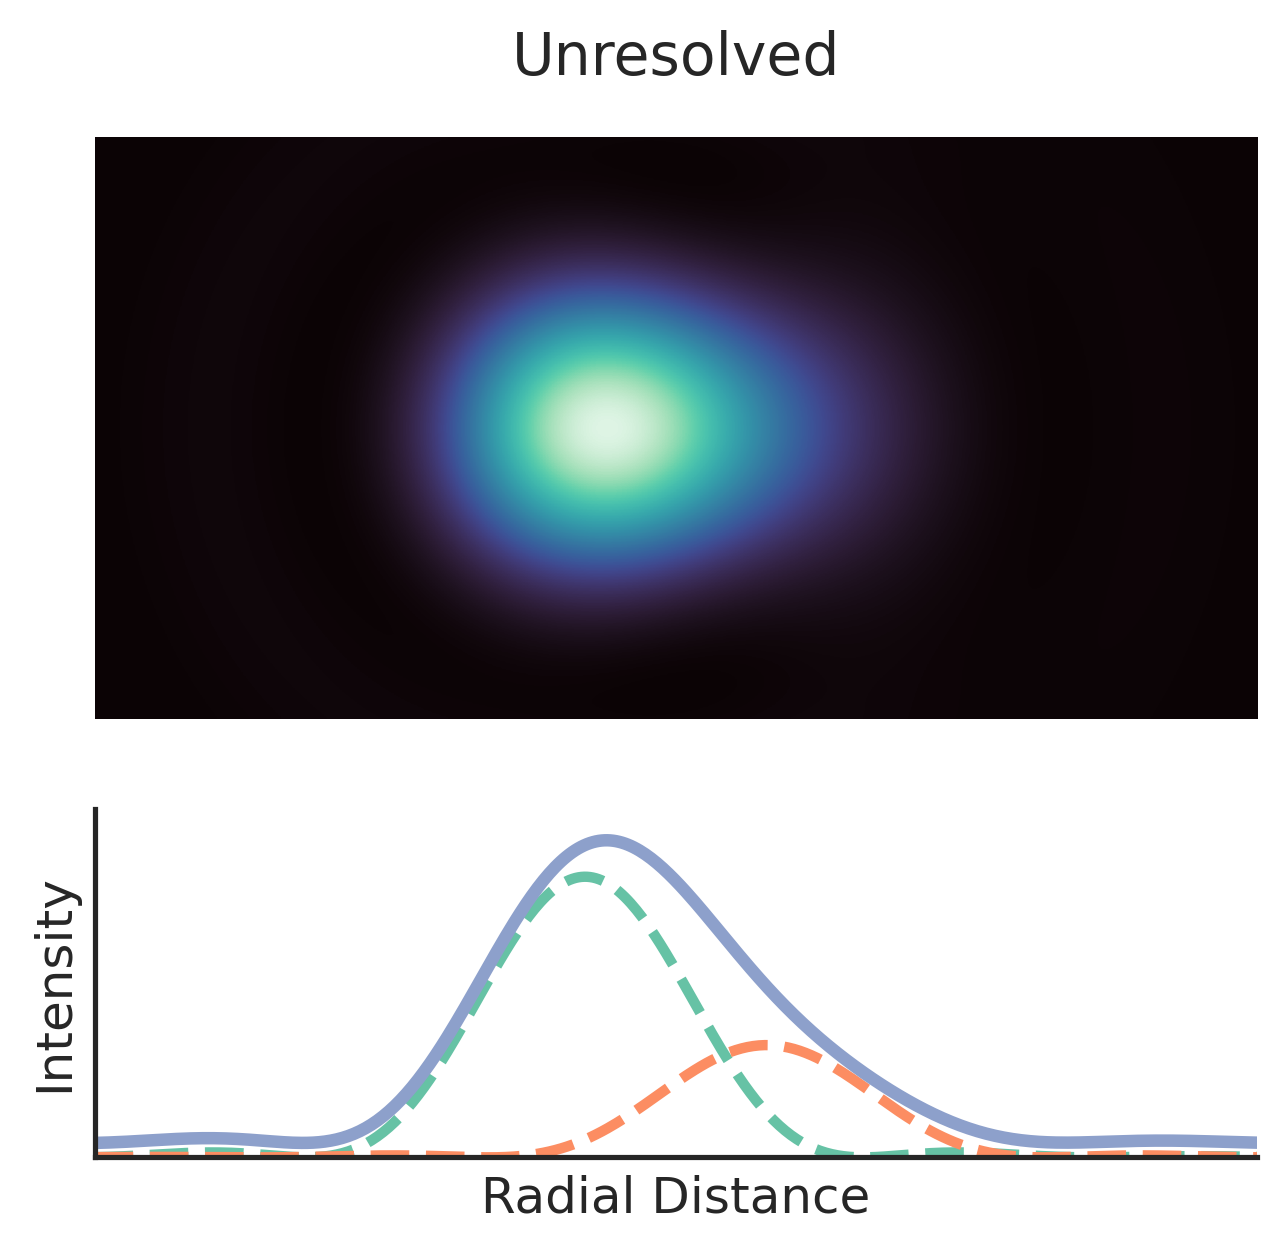
\includegraphics[width=0.48\textwidth]{figures/scripts_for_figures/rayleigh_unresolved.png}
    \caption{Two unequal point sources in a diffraction-limited image. When their separation is large compared with the PSF width (left), two features can be distinguished directly. In the sub-Rayleigh regime (right), the intensity profiles overlap into one dominant feature. The faint source is still present, but its displacement is encoded only as a small change in the combined profile.}
    \label{fig:rayleigh_criterion}
\end{figure}

\begin{remark}[What ``sub-Rayleigh'' means here]
    The Rayleigh criterion is a useful visual rule, not a statement that estimation becomes mathematically impossible below a sharp boundary. The issue is statistical: as the PSFs overlap, an intensity measurement contains progressively less accessible information about the faint source per detected photon. With enough resources a direct image may still reveal it; the required resources can simply become prohibitive at high contrast.
\end{remark}

\section{Why an intensity image is poorly conditioned}

For clarity, consider two incoherent sources separated along the $x$ direction and approximate the PSF by a Gaussian of width $w_0$. Conditional on detecting a photon, direct imaging samples its position from
\begin{equation}
    p_{\mathrm{DI}}(x,y\mid d,\epsilon)
    = \frac{e^{-y^2/(2w_0^2)}}{2\pi w_0^2}
    \left[(1-\epsilon)e^{-x^2/(2w_0^2)}
        +\epsilon e^{-(x-d)^2/(2w_0^2)}\right].
    \label{eq:di_probability_distribution}
\end{equation}
The detector records only this intensity distribution: it does not resolve the optical field into phase-sensitive spatial components. For $d\ll w_0$, changing $d$ changes the image only weakly, while the change is weighted by the already small factor $\epsilon$.

For the known-reference-star model above, the Fisher information per temporal mode therefore has the leading high-contrast behaviour
\begin{equation}
    \mathcal{I}_{\mathrm{DI}}(d) \sim \frac{\eta\epsilon^2}{w_0^2},
    \qquad d\ll w_0,
    \label{eq:di_fisher_collapse}
\end{equation}
where $\eta$ is the probability that a photon is detected in that temporal mode. The important feature is the $\epsilon^2$ dependence: the displacement signal in the intensity image is suppressed twice, once by the faint-source brightness and again when its weak deformation is estimated against the bright background. This high-contrast form of Rayleigh's curse is the limitation that motivates a different measurement basis~\cite{Santamaria2024single,Tsang2016quantum}.

\subsection{How direct-imaging data are normally used}

In a conventional analysis, the detector pixels provide counts sampled from Eq.~\eqref{eq:di_probability_distribution} (or from a more realistic PSF model). A forward model is fitted to those counts to estimate $\boldsymbol d$, $\epsilon$, and any nuisance parameters such as the star position or background. The fit may be formulated as maximum likelihood or Bayesian inference. The statistical issue above is not that these procedures are invalid; it is that their likelihood changes very slowly with the faint-source displacement in the regime of interest.

\section{Weak astronomical light as a spatial quantum state}

The same imaging problem can be described at the single-photon level. In the weak-light regime, a temporal mode is usually vacuum, and a non-vacuum event contains one photon from either incoherent source. Its density operator is
\begin{equation}
    \rho_d=(1-\eta)|0\rangle\langle0|
    +\eta(1-\epsilon)|\psi_0\rangle\langle\psi_0|
    +\eta\epsilon|\psi_d\rangle\langle\psi_d|,
    \label{eq:optical_density_matrix_chap}
\end{equation}
where $|0\rangle$ is the vacuum, $|\psi_0\rangle$ is the spatial state from the star, and $|\psi_d\rangle$ is the shifted spatial state from the planet. The state is normalized. The mixture, rather than a coherent superposition of the two source states, expresses their mutual incoherence.

For the Gaussian PSF used for intuition in this chapter,
\begin{align}
    \langle x,y|\psi_0\rangle
     & =\left(\frac{1}{2\pi w_0^2}\right)^{1/2}
    \exp\!\left[-\frac{x^2+y^2}{4w_0^2}\right],
    \label{eq:star_wavefunction}                \\
    \langle x,y|\psi_d\rangle
     & =\left(\frac{1}{2\pi w_0^2}\right)^{1/2}
    \exp\!\left[-\frac{(x-d_x)^2+(y-d_y)^2}{4w_0^2}\right].
    \label{eq:planet_wavefunction}
\end{align}
This description does not assume that an astronomical field is prepared in a laboratory quantum state. It is a compact statistical description of the spatial degree of freedom carried by each detected photon. It makes explicit that the choice of measurement basis is part of the estimation problem.

\section{SPADE: measuring in spatial modes}

Spatial-mode demultiplexing (SPADE) replaces pixel measurements with projections onto a set of orthogonal transverse modes~\cite{Tsang2016quantum,Santamaria2024single}. The key design choice is to use modes matched to the PSF and to centre the lowest-order mode on the bright source. For a Gaussian PSF, the natural family is the Hermite--Gaussian (HG) basis.

The fundamental mode is the star-centred PSF, while the two first-order modes are its displacement-sensitive directions:
\begin{align}
    |HG_{00}\rangle
     & =\int dx\,dy\,\psi_0(x,y)a^\dagger(x,y)|0\rangle,
    \label{eq:hg00_def}                                               \\
    |HG_{01}\rangle
     & =\int dx\,dy\,\frac{y}{w_0}\psi_0(x,y)a^\dagger(x,y)|0\rangle,
    \label{eq:hg01_def}                                               \\
    |HG_{10}\rangle
     & =\int dx\,dy\,\frac{x}{w_0}\psi_0(x,y)a^\dagger(x,y)|0\rangle.
    \label{eq:hg10_def}
\end{align}
Here $a^\dagger(x,y)$ creates a photon at image-plane position $(x,y)$. A practical mode sorter implements these projections optically and directs the modes to separate photon-counting ports.

\begin{figure}[htbp]
    \centering
    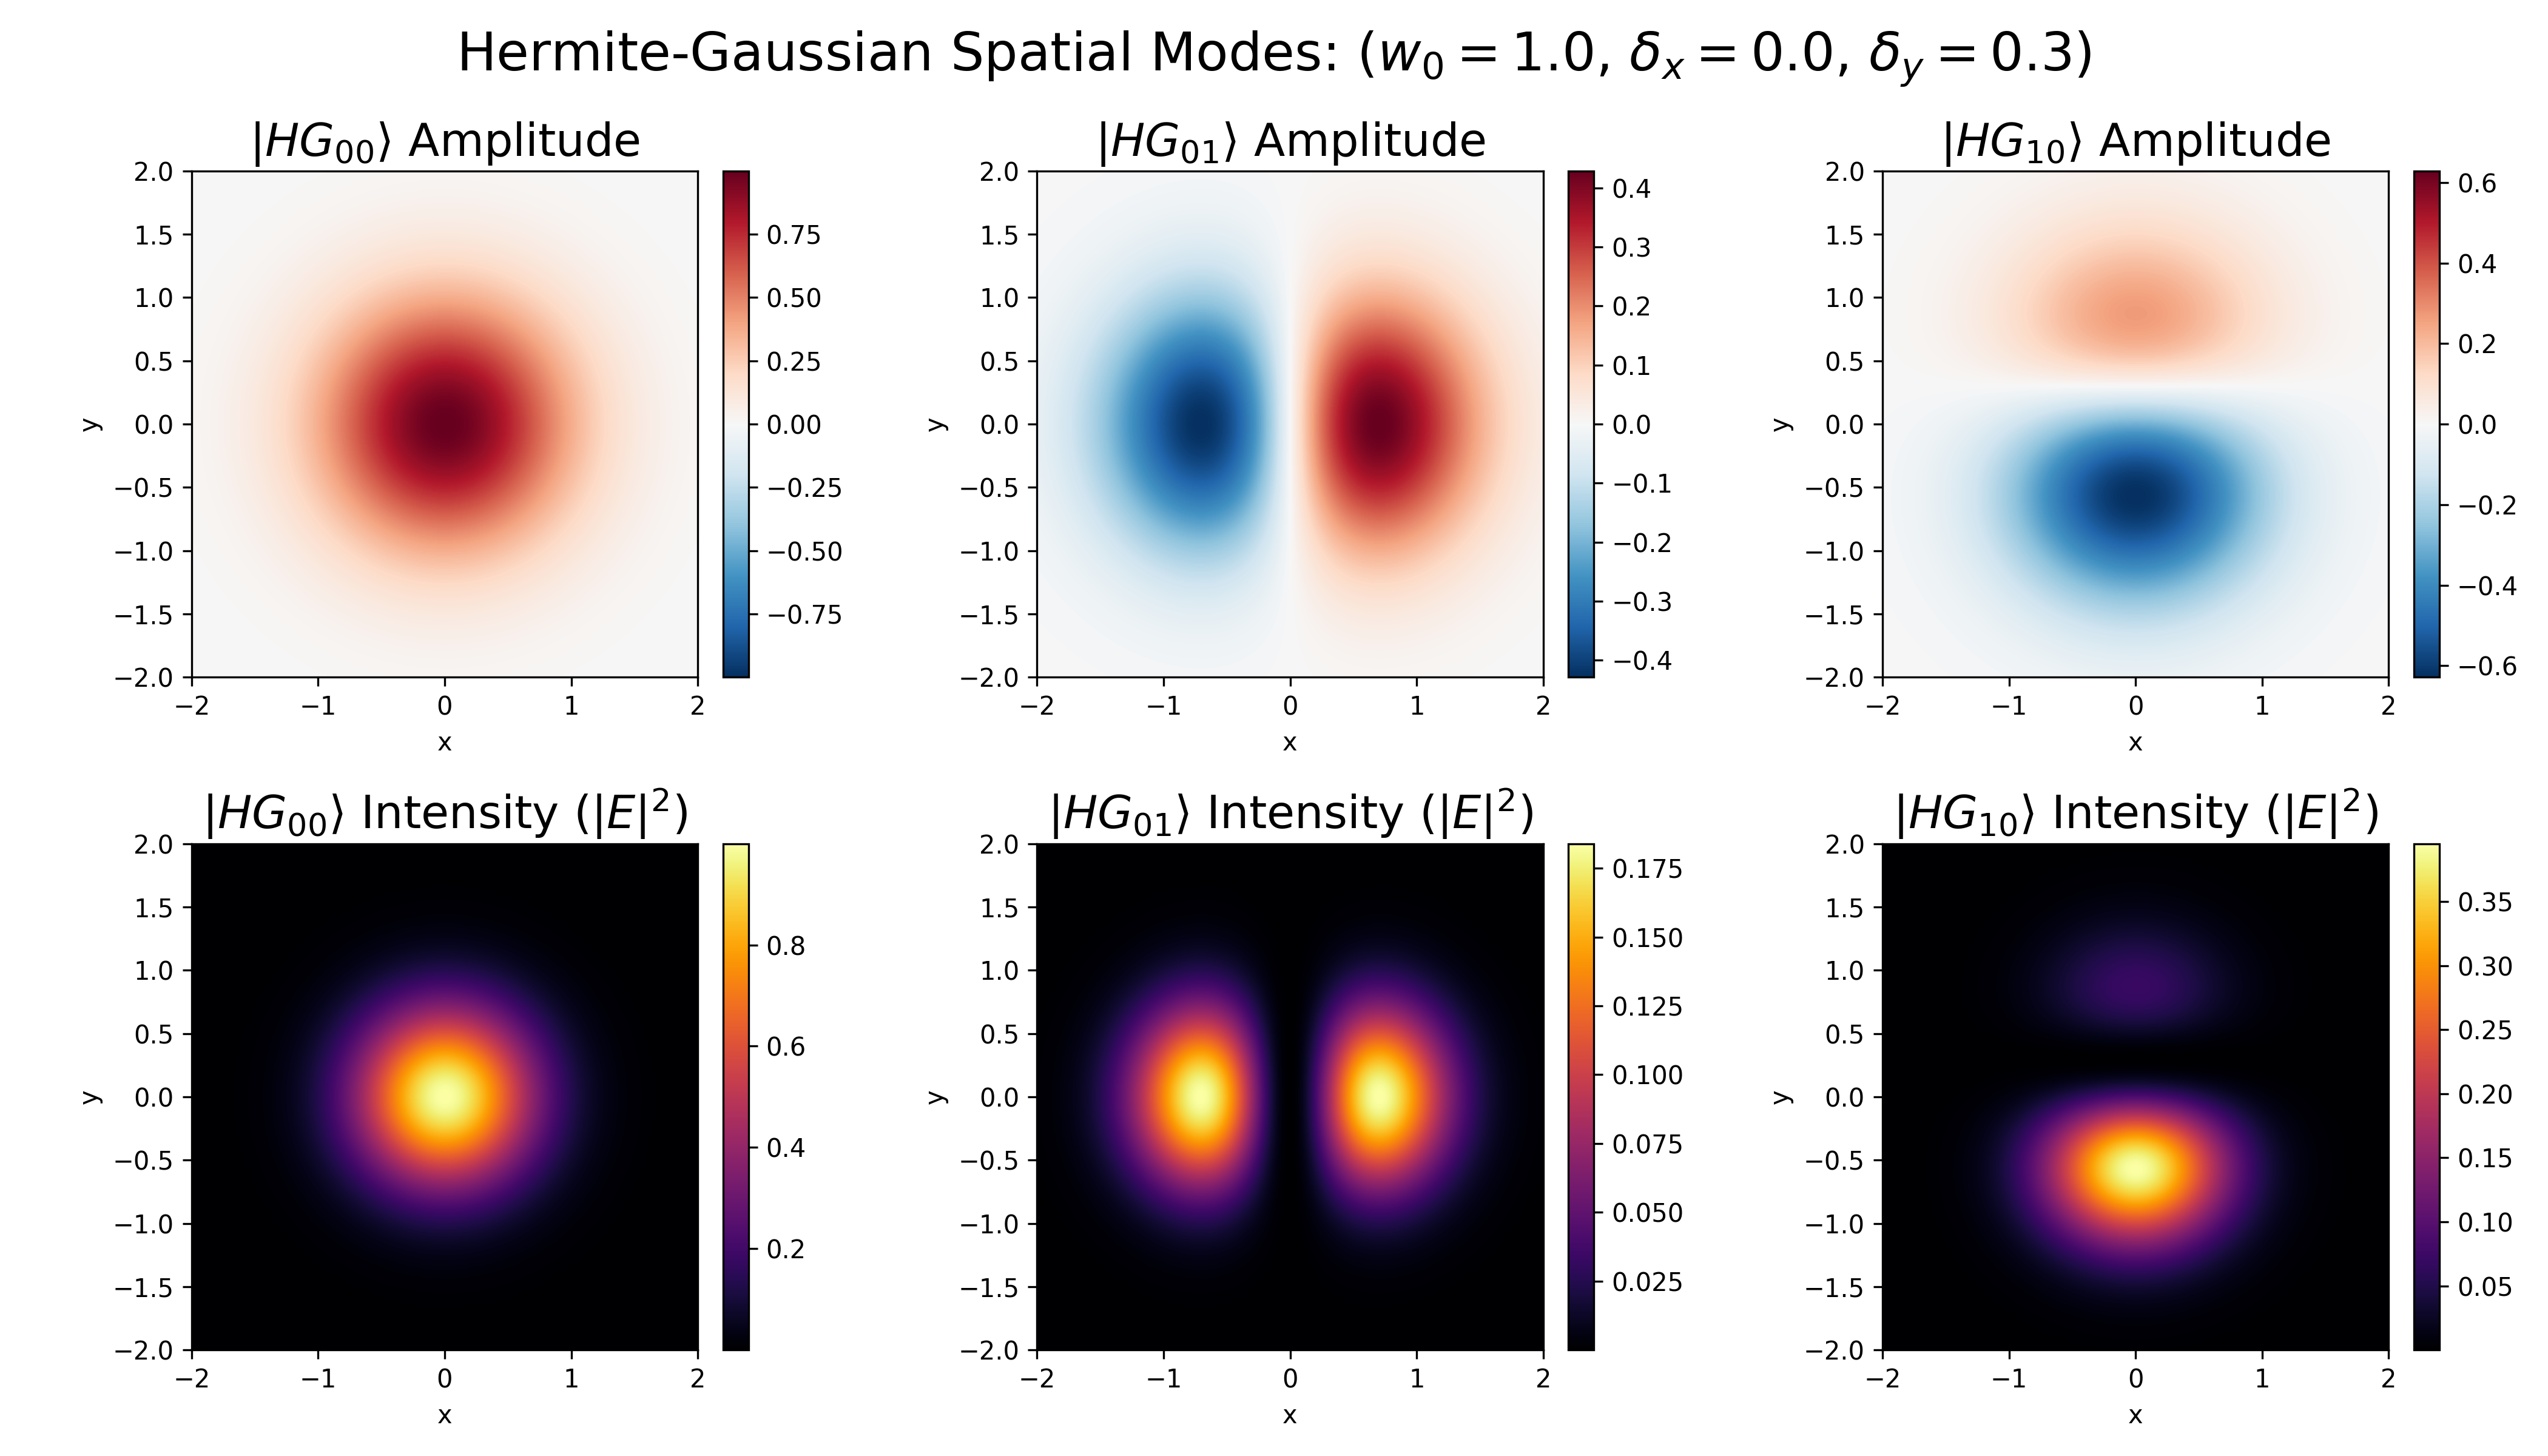
\includegraphics[width=\textwidth]{figures/scripts_for_figures/hg_modes_visualization.png}
    \caption{The fundamental and first-order Hermite--Gaussian spatial modes. The first-order modes have a sign change across one transverse axis, so a small displacement of a PSF away from the fundamental-mode centre transfers amplitude into them.}
    \label{fig:hg_modes}
\end{figure}

It is useful to group the lowest-order ports as
\begin{align}
    \Pi_0 & =|HG_{00}\rangle\langle HG_{00}|,
    \label{eq:pi0_def}                        \\
    \Pi_1 & =|HG_{01}\rangle\langle HG_{01}|
    +|HG_{10}\rangle\langle HG_{10}|.
    \label{eq:pi1_def}
\end{align}
These projectors define a \emph{low-order modal cutoff}, not a spectral-rank truncation of $\rho_d$. That distinction is important for the QFI-based comparison developed later in the thesis.

When the sorter is aligned to the star, the star predominantly occupies $HG_{00}$. A small planetary displacement populates the first-order sector. In the ideal Gaussian model, the probability for a temporal mode to produce a detection in that sector has the leading form
\begin{equation}
    p_1\simeq \eta\epsilon\frac{d_x^2+d_y^2}{4w_0^2},
    \qquad d\ll w_0.
    \label{eq:p1_asymmetric}
\end{equation}
Thus the first-order counts provide a direct displacement-sensitive observable without requiring the planet to form a visually separated intensity peak. Higher-order modes, background rejection, and different modal bases can also be useful; the low-order picture is the simplest illustration of the SPADE principle.

\subsection{Alignment and ordinary SPADE inference}

The required reference frame is normally obtained by centring the fundamental mode on the bright source. With a residual alignment offset $\bmdelta = (\delta_x,\delta_y)$, its single-photon count probability is
\begin{equation}
    p_0=\eta(1-\epsilon)e^{-(\delta_x^2+\delta_y^2)/(4w_0^2)}
    +\eta\epsilon e^{-[(d_x-\delta_x)^2+(d_y-\delta_y)^2]/(4w_0^2)}.
    \label{eq:p0_alignment}
\end{equation}
Maximising this count is a natural star-centric alignment rule. It reduces leakage of the bright star into the displacement-sensitive ports, but it does not by itself estimate the planet parameters.

After alignment, a standard SPADE experiment records the counts in ports such as $HG_{00}$, $HG_{10}$, and $HG_{01}$. These counts, or their relative frequencies, are compared with a calibrated forward model for the modal probabilities. A likelihood fit then estimates $\boldsymbol d$ and/or $\epsilon$; uncertainties arise from finite photon number as well as imperfect alignment, loss, background, and mode cross talk. The details of how those effects are modelled and how QFI is used to assess the resulting procedure belong to the following application chapter, rather than to this physical introduction.

\begin{remark}[Scope of the SPADE advantage]
    SPADE does not remove diffraction, create photons, or make every practical receiver optimal. Its advantage is to access a spatial-mode statistic that is poorly represented in a raw intensity image. Whether that advantage survives in a concrete instrument depends on its alignment, loss, cross talk, photon budget, and the parameters treated as unknown.
\end{remark}

\section{Takeaway}

High-contrast sub-Rayleigh imaging is an estimation problem in which the informative change of a faint source is hidden inside the much larger intensity profile of a bright source. Direct imaging treats the field position by position and becomes poorly conditioned in this regime. SPADE instead sorts the same incoming photons into a PSF-matched spatial basis, where low-order mode populations reveal small displacements. This establishes the physical baseline for the QFI-based method and its experimental implementation developed in the next chapter.
